\documentclass[11pt,class=report,crop=false]{standalone}
\usepackage{exo7hilisit}

\begin{document}


\entete{Hilisit}{Capacité mathématiques}

\titre{\'Equations différentielles -- Partie 1 : Primitives}

\bigskip
\bigskip


%%%%%%%%%%%%%%%%%%%%%%%%%%%%%%%%%%%%%%%%%%%%%%%%%%%%%%%%%%%%
%\section{Primitive}

\exercice{}
\enonce
Mettre en correspondance chaque fonction $f$ avec une de ses primitives $F$. 
 \begin{itemize}
  \item $f_1(x) = -6\sin(2x)$, $f_2(x) = 2x$, $f_3(x) = (x+1)e^x$, $f_4(x) = -6\sin(3x)$, $f_5(x) = 2xe^{x^2}$, $f_6(x)=2x+2$.
  \item $F_a(x) = 2\cos(3x)$, $F_b(x) = 3\cos(2x)$, $F_c(x) = (x+1)^2$, $F_d(x) = x^2+1$, $F_e(x) = e^{x^2}$, $F_f(x) = xe^x$. 
\end{itemize} 
\finenonce

\finexercice


\exercice{}
\enonce
Pour chacune des fonctions $f$ suivantes, déterminer une primitive $F$.
\begin{enumerate}
  \item $f_1(x) = -\cos(2x)$
  \item $f_2(x) = x^3-7x^2+1$
  \item $f_3(x) = \frac{1}{2x-1}$ (sur $]-\frac12,+\infty[$)
  \item $f_4(x) = e^{\pi x-3}$
  \item $f_5(x) = -(x-2)^2$
  \item $f_6(x) = \sin(8(x+1))$
\end{enumerate} 
\finenonce

\finexercice


\exercice{}
\enonce
\sauteligne
\begin{enumerate}
  \item 
  \begin{enumerate}
    \item Quelle est la dérivée de la fonction $x \mapsto u^k(x)$ où $x \mapsto u(x)$ est une fonction et $k$ un entier ?
    \item Calculer les dérivées des fonctions définies par $(x^4+7x^3+2)^3$, $\cos^3(2x)$, $\ln^2(x)$, $\frac{1}{(x^2+1)^2}$.
    \item Déterminer une primitive des fonctions définies par $x(x^2+5)^5$, $\sin(x) \cos^3(x)$, $\frac{\ln^n(x)}{x}$ (où $n\ge0$).
  \end{enumerate} 

  \item 
  \begin{enumerate}
    \item Quelle est la dérivée de la fonction $x \mapsto e^{u(x)}$ où $x \mapsto u(x)$ est une fonction ?
    \item Calculer les dérivées des fonctions définies par $e^{-5x}$, $e^{x^3-2x}$, $e^{\sin(3x)}$, $e^{1/x}$.
    \item Déterminer une primitive des fonctions définies par $e^{8x+1}$, $xe^{x^2+1}$, $\frac{e^{\sqrt x}}{\sqrt x}$.
  \end{enumerate} 


  \item 
  \begin{enumerate}
    \item Quelle est la dérivée de la fonction $x \mapsto \ln(u(x))$ où $x \mapsto u(x)$ est une fonction strictement positive ?
    \item Calculer les dérivées des fonctions définies par $\ln(x^3-2)$, $\ln(e^x+e^{-x})$, $\ln(1/x)$, $\ln(\cos(x^2))$.
    \item Déterminer une primitive des fonctions définies par $\frac{1}{x+4}$ (sur $]-4,+\infty[$), $\frac{x}{x^2+4}$ (sur $\Rr$), $\frac{\cos(x)}{\sin(x)}$ (pour les $x$ où $\sin(x)>0$).
  \end{enumerate} 

\end{enumerate} 
\finenonce

\finexercice


\exercice{}
\enonce
\sauteligne
 \begin{enumerate}
  \item Pour la fonction $f$ représentée ci-dessous, déterminer quel est le graphe de la fonction $F_i$ qui correspond à une primitive de $f$.
\begin{center}
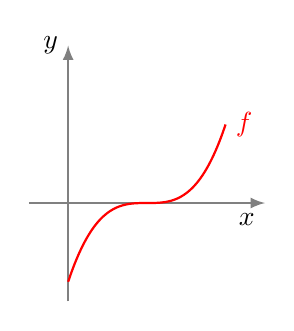
\begin{tikzpicture}[scale=1]
  \draw[->,>=latex,thick,gray] (-0.5,0) -- (2.5,0) node[below left,black] {$x$};
  \draw[->,>=latex,thick,gray] (0,-1.25) -- (0,2) node[left,black] {$y$};
  \draw[thick, color=red,domain=0:2, smooth,samples=50] plot (\x,{(\x-1)^3}) node[right]{$f$};
\end{tikzpicture}
\end{center}

\begin{center}
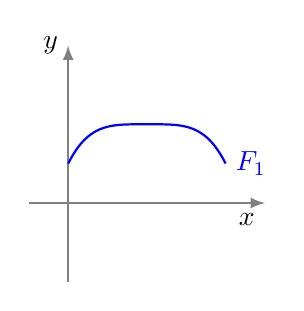
\begin{tikzpicture}[scale=1]
  \draw[->,>=latex,thick,gray] (-0.5,0) -- (2.5,0) node[below left,black] {$x$};
  \draw[->,>=latex,thick,gray] (0,-1) -- (0,2) node[left,black] {$y$};
  \draw[thick, color=blue,domain=0:2, smooth,samples=50] plot (\x,{-1/2*(\x-1)^4+1}) node[right]{$F_1$};
\end{tikzpicture}
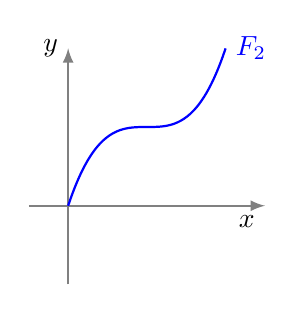
\begin{tikzpicture}[scale=1]
  \draw[->,>=latex,thick,gray] (-0.5,0) -- (2.5,0) node[below left,black] {$x$};
  \draw[->,>=latex,thick,gray] (0,-1) -- (0,2) node[left,black] {$y$};
  \draw[thick, color=blue,domain=0:2, smooth,samples=50] plot (\x,{(\x-1)^3+1}) node[right]{$F_2$};
\end{tikzpicture}
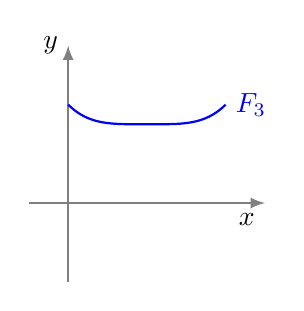
\begin{tikzpicture}[scale=1]
  \draw[->,>=latex,thick,gray] (-0.5,0) -- (2.5,0) node[below left,black] {$x$};
  \draw[->,>=latex,thick,gray] (0,-1) -- (0,2) node[left,black] {$y$};
  \draw[thick, color=blue,domain=0:2, smooth,samples=50] plot (\x,{1/4*(\x-1)^4+1}) node[right]{$F_3$};
\end{tikzpicture}
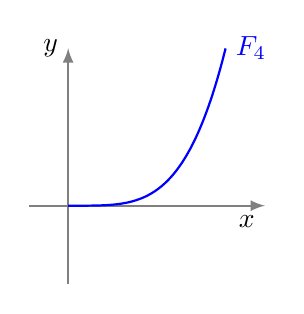
\begin{tikzpicture}[scale=1]
  \draw[->,>=latex,thick,gray] (-0.5,0) -- (2.5,0) node[below left,black] {$x$};
  \draw[->,>=latex,thick,gray] (0,-1) -- (0,2) node[left,black] {$y$};
  \draw[thick, color=blue,domain=0:2, smooth,samples=50] plot (\x,{1/8*\x^4}) node[right]{$F_4$};
\end{tikzpicture}
\end{center}

  \item Pour la fonction $f$ représentée ci-dessous, déterminer quel est le graphe de la fonction $F_i$ qui correspond à une primitive de $f$.
\begin{center}
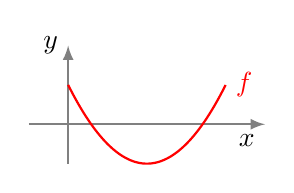
\begin{tikzpicture}[scale=1]
  \draw[->,>=latex,thick,gray] (-0.5,0) -- (2.5,0) node[below left,black] {$x$};
  \draw[->,>=latex,thick,gray] (0,-0.5) -- (0,1) node[left,black] {$y$};
  \draw[thick, color=red,domain=0:2, smooth,samples=50] plot (\x,{(\x-1)^2-1/2}) node[right]{$f$};
\end{tikzpicture}
\end{center}

\begin{center}
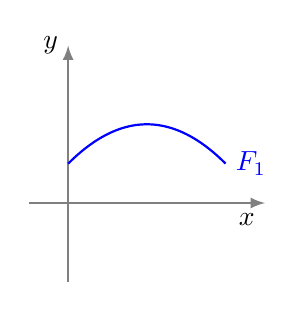
\begin{tikzpicture}[scale=1]
  \draw[->,>=latex,thick,gray] (-0.5,0) -- (2.5,0) node[below left,black] {$x$};
  \draw[->,>=latex,thick,gray] (0,-1) -- (0,2) node[left,black] {$y$};
  \draw[thick, color=blue,domain=0:2, smooth,samples=50] plot (\x,{-1/2*(\x-1)^2+1}) node[right]{$F_1$};
\end{tikzpicture}
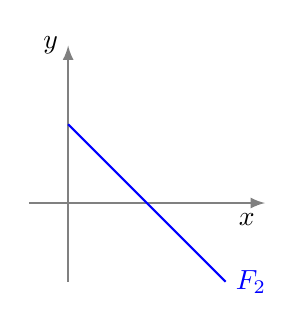
\begin{tikzpicture}[scale=1]
  \draw[->,>=latex,thick,gray] (-0.5,0) -- (2.5,0) node[below left,black] {$x$};
  \draw[->,>=latex,thick,gray] (0,-1) -- (0,2) node[left,black] {$y$};
  \draw[thick, color=blue,domain=0:2, smooth,samples=50] plot (\x,{-\x+1}) node[right]{$F_2$};
\end{tikzpicture}
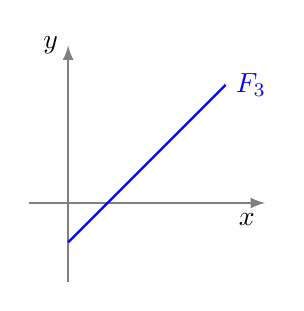
\begin{tikzpicture}[scale=1]
  \draw[->,>=latex,thick,gray] (-0.5,0) -- (2.5,0) node[below left,black] {$x$};
  \draw[->,>=latex,thick,gray] (0,-1) -- (0,2) node[left,black] {$y$};
  \draw[thick, color=blue,domain=0:2, smooth,samples=50] plot (\x,{\x-0.5}) node[right]{$F_3$};
\end{tikzpicture}
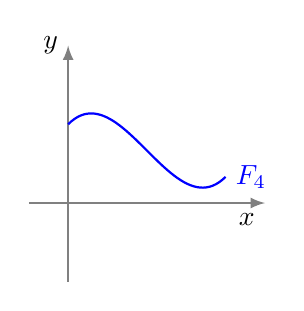
\begin{tikzpicture}[scale=1]
  \draw[->,>=latex,thick,gray] (-0.5,0) -- (2.5,0) node[below left,black] {$x$};
  \draw[->,>=latex,thick,gray] (0,-1) -- (0,2) node[left,black] {$y$};
  \draw[thick, color=blue,domain=0:2, smooth,samples=50] plot (\x,{2*(\x/2 - \x^2 + \x^3/3)+1}) node[right]{$F_4$};
\end{tikzpicture}
\end{center}

\end{enumerate} 
\finenonce

\end{document}
